\documentclass[10pt,conference]{IEEEtran}
\usepackage[T1]{fontenc}
\usepackage[utf8]{inputenc}
\usepackage{times,amsmath,graphicx,booktabs,url}
\graphicspath{{figures/}}
\title{Visualisasi dan Analisis Prediksi Penyewaan Sepeda Berbasis Time-Series Menggunakan Convolutional Neural Network}
\author{\IEEEauthorblockN{Nathanael Gunawan (13524066) dan Audric Yusuf Maynard Simatupang (13524010)}
\IEEEauthorblockA{Program Studi Teknik Informatika\\Sekolah Teknik Elektro dan Informatika, Institut Teknologi Bandung}}
\begin{document}
\maketitle
\begin{abstract}
Studi ini menganalisis pola penyewaan sepeda dan hasil prediksi satu jam ke depan menggunakan CNN satu dimensi pada Bike Sharing Dataset. Dua konfigurasi dibandingkan: univariat yang menggunakan riwayat jumlah penyewaan dan multivariat yang menambahkan temperatur, kelembapan, serta kecepatan angin. Input berupa jendela 24 jam dengan pembagian data secara kronologis. Analisis terhadap hasil eksperimen tersimpan pada 2.261 target uji menunjukkan MAE sebesar 35,64 dan RMSE 53,80 untuk model univariat, sedangkan model multivariat mencapai MAE 34,34 dan RMSE 50,85. Penurunan kesalahan tersebut bersifat moderat dan tidak merata: kesalahan terbesar masih muncul pada pukul 08.00 dan 17.00. Visualisasi menunjukkan pentingnya mengevaluasi model berdasarkan waktu, bias, dan kesalahan ekstrem selain metrik agregat. Temuan terbatas pada satu konfigurasi dan satu seed sehingga belum membuktikan keunggulan yang konsisten di seluruh periode atau pelatihan ulang.
\end{abstract}
\begin{IEEEkeywords}
time-series, CNN, penyewaan sepeda, visualisasi, prediksi.
\end{IEEEkeywords}

\section{Pendahuluan}
Jumlah penyewaan sepeda berubah sepanjang waktu. Pola harian, perbedaan hari kerja dan hari libur, serta kondisi lingkungan dapat menyertai perubahan permintaan. Visualisasi membantu mengenali pola tersebut sekaligus menunjukkan kondisi ketika prediksi model menyimpang dari observasi.

Penelitian ini menggunakan data penyewaan per jam untuk menjawab tiga pertanyaan: bagaimana pola permintaan berbeda menurut jam dan jenis hari; apakah penambahan variabel cuaca historis memperbaiki prediksi CNN; serta pada kondisi waktu apa model menghasilkan kesalahan terbesar. CNN digunakan sebagai model prediksi, sedangkan grafik deret waktu, kurva pelatihan, dan kesalahan per jam digunakan untuk menginterpretasikan data dan hasil model.

\section{Dataset dan Persiapan Data}
\subsection{Sumber dan variabel}
Bike Sharing Dataset memuat data Capital Bikeshare di Washington, D.C., pada 2011--2012 beserta atribut kalender dan lingkungan \cite{dataset}. Berkas \texttt{hour.csv} memiliki 17.379 observasi. Target \texttt{cnt} menyatakan total penyewaan dalam satu jam, bukan jumlah pengguna unik. Model univariat memakai \texttt{cnt}; model multivariat memakai \texttt{cnt}, \texttt{temp}, \texttt{hum}, dan \texttt{windspeed}. Temperatur, kelembapan, dan angin merupakan atribut ternormalisasi pada dataset. Atribut \texttt{workingday} digunakan untuk analisis deskriptif, tetapi tidak menjadi input kedua model.

\subsection{Kualitas dan pembagian kronologis}
Timestamp dibentuk dari tanggal dan jam. Metadata eksperimen mencatat tidak ada nilai kosong atau timestamp duplikat, tetapi terdapat 75 jeda temporal yang mencakup 165 jam tanpa observasi. Tidak adanya nilai kosong pada baris yang tersedia tidak berarti seluruh jam kalender tersedia. Jendela input yang melintasi jeda waktu dikeluarkan, tanpa mengisi jam yang hilang dengan nol.

Sebanyak 13.000 baris pertama digunakan untuk pelatihan, 2.000 berikutnya untuk validasi, dan 2.379 terakhir untuk pengujian. Pelatihan berakhir pada 30 Juni 2012 pukul 20.00; validasi berlangsung hingga 22 September 2012 pukul 04.00; periode uji dimulai satu jam setelahnya dan berakhir 31 Desember 2012 pukul 23.00. Setelah pembentukan jendela, jumlah sampel efektif adalah 11.396, 2.000, dan 2.261. Jumlah baris mentah berbeda dari jumlah pasangan input--target yang dapat digunakan.

MinMaxScaler untuk fitur dan target hanya di-fit pada data pelatihan. Parameter yang sama diterapkan pada validasi dan pengujian. Target menentukan keanggotaan split; konteks input dapat berasal dari periode sebelumnya. Evaluasi bersifat rolling satu langkah: observasi aktual yang sudah tersedia dapat digunakan untuk memprediksi jam berikutnya. Hasil ini tidak mewakili prediksi rekursif untuk banyak jam sekaligus.

\section{Metode}
\subsection{Arsitektur CNN}
Untuk target pada jam $t$, input terdiri atas 24 observasi berurutan sebelum $t$. Dimensi input adalah $24\times1$ pada univariat dan $24\times4$ pada multivariat. Konvolusi satu dimensi memproses pola lokal sepanjang sumbu waktu melalui filter yang parameternya dipelajari. Arsitektur implementasi terdiri atas Conv1D dengan 32 filter dan kernel 3, ReLU, Flatten, Dense 16 dengan ReLU, serta Dense 1 linear. Konvolusi menggunakan padding valid. Lapisan keluaran linear memungkinkan prediksi bernilai negatif sehingga kelayakan nilai keluaran juga perlu diperiksa.

Kedua konfigurasi menggunakan Adam, loss MSE, batch size 32, batas 50 epoch, dan seed 42. Data pelatihan tidak diacak. Early stopping memantau loss validasi dengan patience 10 dan mengembalikan bobot pada epoch validasi terbaik. Model univariat selesai pada epoch 32 dengan epoch terbaik 22; model multivariat selesai pada epoch 31 dengan epoch terbaik 21.

\subsection{Evaluasi dan asal hasil}
Paper ini menganalisis artefak eksperimen yang telah tersimpan pada repositori \cite{repo}: metadata dan riwayat pelatihan, serta CSV prediksi pengujian. Angka MAE dan RMSE dihitung ulang dari CSV; nilai aktual dicocokkan dengan dataset dan timestamp kedua model diperiksa agar perbandingan menggunakan target identik. Analisis ini tidak melakukan pelatihan ulang. Grafik disusun kembali dari data dan artefak tersebut.

Dengan $e_i=\hat y_i-y_i$, metrik utama adalah
\begin{equation}
\operatorname{MAE}=\frac{1}{n}\sum_{i=1}^{n}|e_i|,\qquad
\operatorname{RMSE}=\sqrt{\frac{1}{n}\sum_{i=1}^{n}e_i^2}.
\end{equation}
Bias merupakan rata-rata $e_i$; nilai positif berarti prediksi cenderung lebih tinggi. MAE, RMSE, dan bias dilaporkan dalam satuan jumlah penyewaan. Loss pelatihan menggunakan target ternormalisasi sehingga nilainya tidak dapat dibandingkan langsung dengan RMSE dalam satuan asli.

\section{Hasil dan Pembahasan}
\subsection{Pola permintaan harian}
Profil rata-rata penyewaan per jam menurut status hari kerja ditunjukkan pada Gambar~\ref{fig:pola}. Agregasi seluruh periode ini merupakan eksplorasi deskriptif, bukan evaluasi model. Perbedaan bentuk profil memperlihatkan bahwa jam yang sama dapat memiliki konteks permintaan berbeda menurut jenis hari. Atribut kalender berpotensi membantu model membedakan konteks tersebut; manfaatnya masih perlu diuji karena belum dimasukkan ke konfigurasi saat ini. Pola agregat tidak cukup untuk menetapkan penyebab perilaku pengguna.
\begin{figure*}[t]
\centering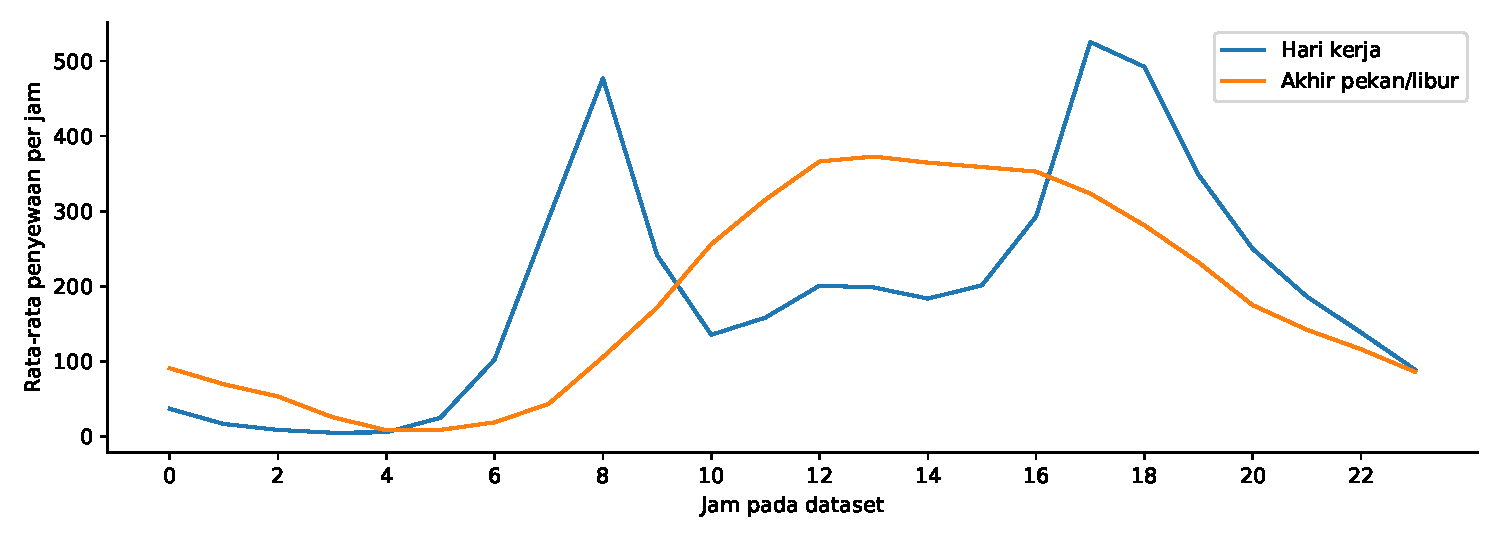
\includegraphics[width=.95\textwidth]{pola_harian.pdf}
\caption{Rata-rata penyewaan per jam pada seluruh dataset, dipisahkan menurut hari kerja dan akhir pekan/libur. Jam mengikuti timestamp dataset tanpa konversi zona waktu.}\label{fig:pola}
\end{figure*}

\subsection{Perbandingan kinerja keseluruhan}
Tabel~\ref{tab:hasil} merangkum evaluasi pada 2.261 target yang sama. Penambahan fitur cuaca historis menurunkan MAE sekitar 3,66\% dan RMSE sekitar 5,47\%. Bias positif berkurang dari 10,54 menjadi 5,84. Dengan demikian, model multivariat memiliki kesalahan rata-rata lebih rendah dalam eksperimen ini, tetapi peningkatannya relatif kecil.
\begin{table}[ht]
\centering\caption{Hasil pengujian dalam satuan penyewaan, kecuali $R^2$.}\label{tab:hasil}
\begin{tabular}{lrr}\toprule
Metrik & Univariat & Multivariat\\\midrule
MAE &35,64&34,34\\
RMSE &53,80&50,85\\
Bias &10,54&5,84\\
$R^2$ &0,9350&0,9419\\
Persentil 95 galat absolut &116,78&106,33\\
Galat absolut maksimum &335,89&396,63\\
Jumlah prediksi negatif &11&26\\\bottomrule
\end{tabular}
\end{table}
Keunggulan rata-rata tidak berlaku untuk semua ukuran. Median galat absolut multivariat adalah 22,76, lebih tinggi daripada univariat sebesar 20,86. Galat absolut maksimumnya juga lebih besar. Sebaliknya, persentil 95 galat absolut lebih rendah. Kombinasi ini menunjukkan bahwa distribusi kesalahan berubah, sehingga satu metrik tidak cukup untuk menyatakan model selalu lebih baik. Perbandingan ini tidak mengisolasi efek masing-masing variabel cuaca dan tidak membuktikan hubungan sebab-akibat.

\subsection{Prediksi terhadap waktu}
Gambar~\ref{fig:pred} menampilkan 168 target uji pertama dengan aturan pemilihan tetap untuk memudahkan pembacaan pola lokal. Rentang pendek membantu melihat waktu puncak dan selisih amplitudo yang dapat tertutup pada grafik seluruh periode. Kesimpulan numerik tetap menggunakan seluruh 2.261 target, bukan hanya cuplikan ini.
\begin{figure*}[t]
\centering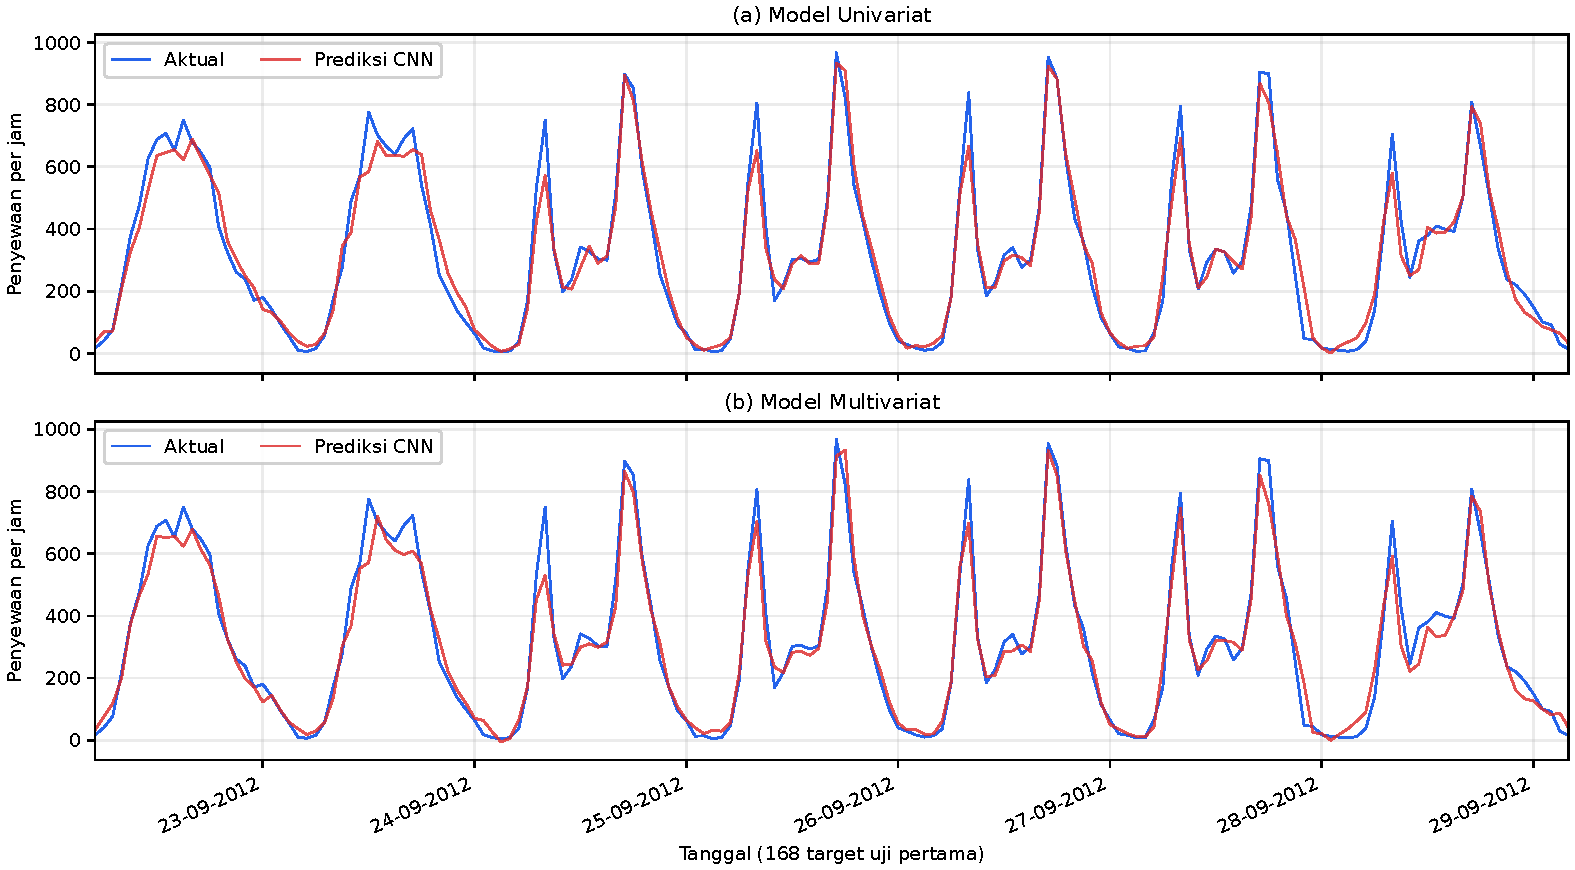
\includegraphics[width=.98\textwidth]{prediksi_minggu.pdf}
\caption{Aktual dan prediksi kedua CNN pada 168 target uji pertama. Cuplikan ini merupakan ilustrasi lokal; metrik dihitung pada seluruh target uji.}\label{fig:pred}
\end{figure*}

\subsection{Kesalahan terkonsentrasi pada jam tertentu}
Pada model univariat, MAE pukul 08.00 mencapai 90,41 dan pukul 17.00 mencapai 86,32. Model multivariat menurunkannya menjadi 79,80 dan 74,86. Keduanya tetap merupakan dua jam dengan MAE tertinggi untuk masing-masing model. Kesalahan pada jam tersebut jauh lebih besar daripada MAE agregat, sehingga angka rata-rata keseluruhan dapat menyamarkan kelemahan pada periode permintaan yang berubah tajam.

\begin{figure*}[t]
\centering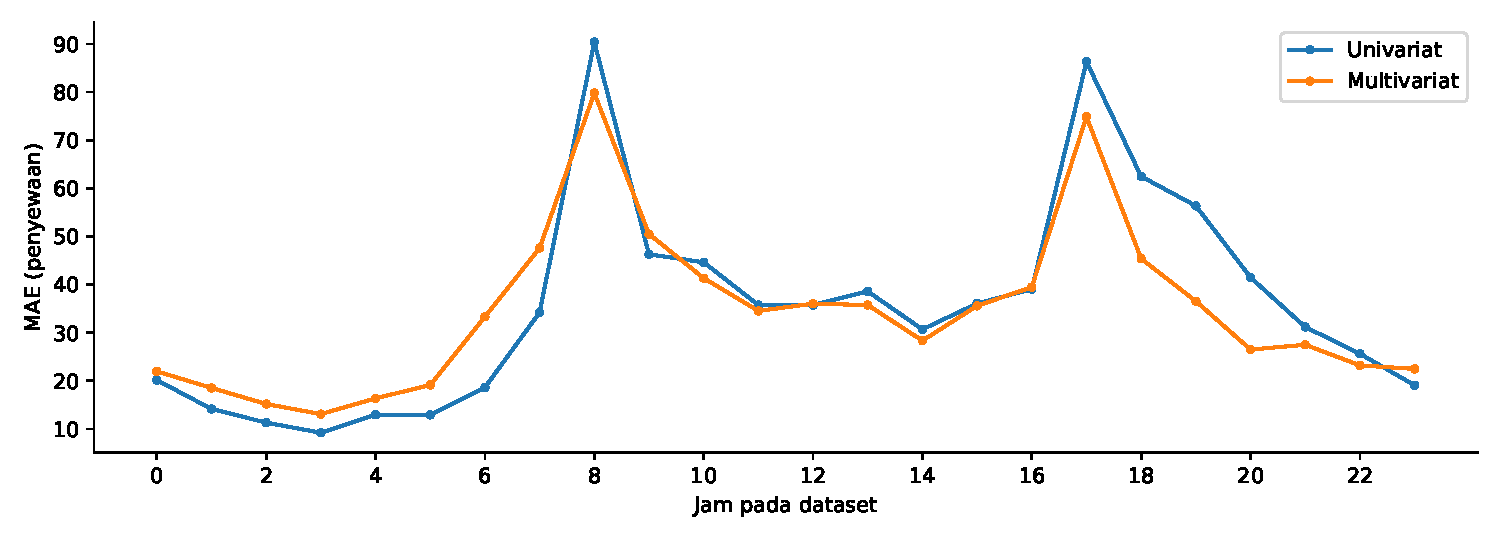
\includegraphics[width=.95\textwidth]{error_per_jam.pdf}
\caption{MAE berdasarkan jam dalam sehari pada target uji yang tersedia. Setiap titik menggabungkan jam yang sama dari berbagai tanggal, bukan urutan 24 jam tertentu.}\label{fig:jam}
\end{figure*}
Temuan ini mendukung evaluasi berdasarkan jam apabila prediksi digunakan untuk perencanaan ketersediaan sepeda. Penggunaan fitur jam, jenis hari, atau loss yang memberikan perhatian pada periode sibuk dapat menjadi eksperimen lanjutan. Pemilihan konfigurasi lanjutan harus menggunakan validasi agar periode uji tidak menjadi dasar penyetelan berulang.

\subsection{Pelatihan dan batas keluaran}
Gambar~\ref{fig:loss} memperlihatkan loss pelatihan dan validasi dalam skala normalisasi. Early stopping memilih bobot berdasarkan validasi, bukan epoch terakhir atau nilai uji. Nilai loss validasi terbaik adalah sekitar 0,002758 untuk univariat dan 0,002622 untuk multivariat. Kurva ini membantu memeriksa proses optimasi, tetapi tidak menggantikan evaluasi pada periode uji yang terpisah.
\begin{figure*}[t]
\centering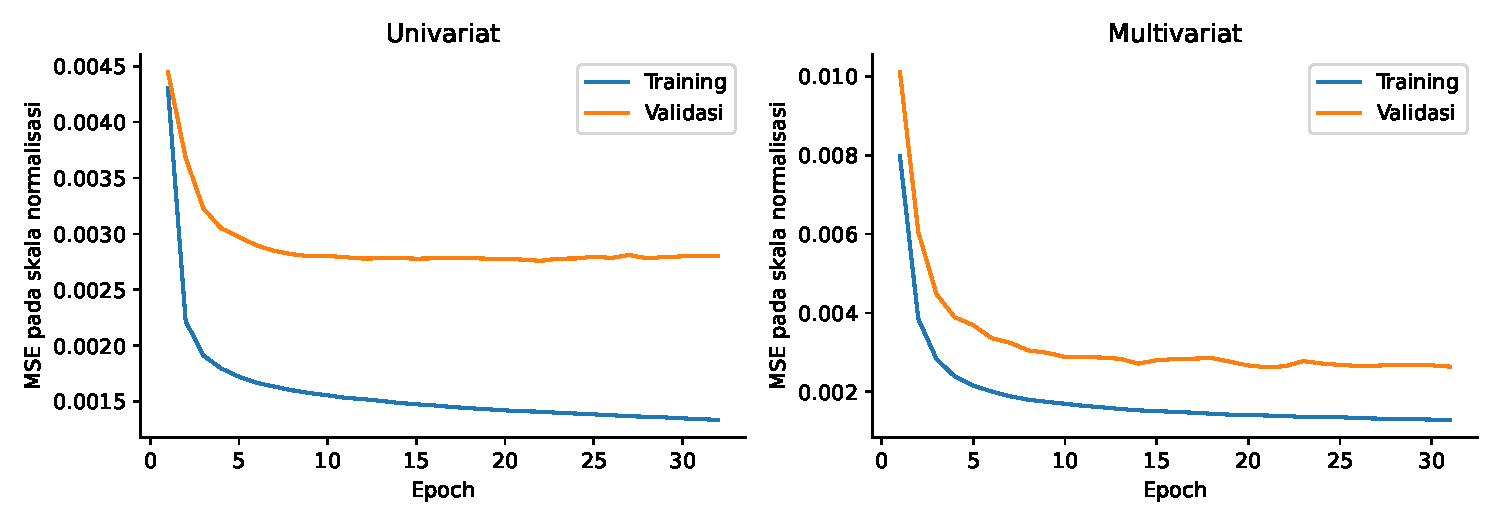
\includegraphics[width=.98\textwidth]{training.pdf}
\caption{Riwayat MSE pelatihan dan validasi. Skala target telah dinormalisasi; panjang pelatihan kedua model berbeda akibat early stopping.}\label{fig:loss}
\end{figure*}
Prediksi negatif ditemukan sebanyak 11 pada univariat dan 26 pada multivariat, dengan nilai minimum masing-masing $-7{,}88$ dan $-17{,}20$. Nilai tersebut tidak sesuai makna fisik jumlah penyewaan. Evaluasi di sini mempertahankan keluaran asli tanpa pembulatan atau clipping. Pembatasan keluaran nonnegatif dapat diuji sebagai perbaikan, tetapi metrik setelah perubahan harus dihitung ulang dan dibedakan dari hasil saat ini.

\section{Keterbatasan}
Eksperimen menggunakan satu seed, satu ukuran jendela, dan satu periode uji sehingga variasi antarpelatihan belum diukur. Baseline sederhana seperti persistence atau prediksi berdasarkan jam yang sama pada hari sebelumnya belum dibandingkan dalam paper ini; hasil belum menunjukkan apakah CNN lebih baik daripada metode sederhana tersebut. Pembagian kronologis juga berarti karakteristik musim pada setiap split tidak identik.

Jendela yang melintasi jam hilang dikeluarkan. Karena itu, metrik berlaku pada target yang memenuhi syarat dan tidak otomatis mewakili seluruh jam kalender. Data agregat satu sistem pada 2011--2012 tidak cukup untuk menggeneralisasi ke kota atau tahun lain. Variabel cuaca yang dipakai berasal dari riwayat input; model tidak menggunakan cuaca aktual masa depan. Perbedaan kinerja kedua konfigurasi belum diuji signifikansinya.

\section{Kesimpulan}
Visualisasi memberi konteks terhadap hasil CNN: profil permintaan berbeda menurut waktu dan jenis hari, sementara kesalahan prediksi tidak tersebar merata sepanjang hari. Pada target uji yang sama, konfigurasi multivariat menurunkan MAE dari 35,64 menjadi 34,34 dan RMSE dari 53,80 menjadi 50,85. Peningkatan rata-rata ini disertai keterbatasan berupa galat maksimum lebih besar, median galat absolut lebih tinggi, dan prediksi negatif lebih banyak.

Insight utama adalah perlunya menilai model melalui pola temporal dan distribusi kesalahan selain skor keseluruhan. Pukul 08.00 dan 17.00 tetap menjadi bagian yang paling sulit bagi kedua konfigurasi. Penelitian lanjutan dapat menguji fitur kalender, baseline sederhana, dan pengulangan pelatihan sebelum menyimpulkan keunggulan CNN multivariat secara lebih luas.

\begin{thebibliography}{2}
\raggedright
\bibitem{dataset} H. Fanaee-T, ``Bike Sharing Dataset,'' UCI Machine Learning Repository, 2013. Dokumentasi dataset lokal: \path{data/bike+sharing+dataset/Readme.txt}.
\bibitem{repo} Tim proyek, ``CNNVisSiscer,'' kode sumber dan artefak eksperimen lokal, evaluasi 4 November 2026. Berkas: \path{src/train/model.py}, \path{src/train/evaluate.py}, serta direktori \path{output/model} dan \path{output/test_output}.
\end{thebibliography}
\end{document}
